% Created 2022-03-25 Fri 15:37
% Intended LaTeX compiler: pdflatex
\documentclass[11pt]{article}
\usepackage[utf8]{inputenc}
\usepackage[T1]{fontenc}
\usepackage{graphicx}
\usepackage{longtable}
\usepackage{wrapfig}
\usepackage{rotating}
\usepackage[normalem]{ulem}
\usepackage{amsmath}
\usepackage{amssymb}
\usepackage{capt-of}
\usepackage{hyperref}
\usepackage{gensymb}
\usepackage{circuitikz}
\usepackage{tikz}
\usepackage{minted}
\usepackage[margin=2cm]{geometry}
\usepackage{fancyhdr}
\pagestyle{fancy}
\fancyhf{}
\fancyhead[L]{{\textcolor{gray}\leftmark}}
\fancyhead[R]{{\textcolor{gray}\thepage}}
\renewcommand{\headrulewidth}{0pt}
\usepackage{url}
\usepackage{rotfloat}
\usepackage{tikz}
\usepackage{float}
\hypersetup{hidelinks}
\usepackage{gensymb}
\usepackage{amsmath}
\numberwithin{equation}{section}
\usepackage{chngcntr}
\counterwithin{figure}{section}
\counterwithin{table}{section}
\usepackage{amssymb}
\newcommand {\R}{\mathbb{R}}
\usepackage{gensymb}
\usepackage{booktabs}
\usepackage{minted}[linenos]
\usepackage{sourcecodepro}
\definecolor{deepblue}{rgb}{0.0, 0.18, 0.39}
\setlength{\parindent}{0}
\usepackage{parskip}
\usepackage{enumitem}
\setlist{noitemsep}
\usepackage[format=plain, labelfont={bf}, textfont=it]{caption}
\usepackage{booktabs}
\usepackage[framemethod=tikz]{mdframed}
\BeforeBeginEnvironment{minted}{\begin{mdframed}[style=sourcecode]}
\AfterEndEnvironment{minted}{\end{mdframed}}
\author{Ben Frazer\thanks{2704250F@student.gla.ac.uk}}
\date{\today}
\title{Robust Control Lab Report}
\hypersetup{
 pdfauthor={Ben Frazer},
 pdftitle={Robust Control Lab Report},
 pdfkeywords={},
 pdfsubject={},
 pdfcreator={Emacs 27.2 (Org mode 9.6)}, 
 pdflang={English}}
\begin{document}

\maketitle
\mdfdefinestyle{sourcecode}{%
%backgroundcolor=darkgray,
skipabove=12pt,
hidealllines=true,
apptotikzsetting={%
  \tikzset{mdfbackground/.append style={fill=deepblue,fill opacity=0.1}}},
leftline=true,%innerleftmargin=10,innerrightmargin=10,
innerleftmargin=25,
linewidth = 4pt,
roundcorner = 2pt,
linecolor= darkgray,
%#frametitlerule=true,frametitlerulecolor=green,
%#frametitlebackgroundcolor=darkgray,
%#frametitlerulewidth=2pt
}


\section{Introduction}
\label{sec:org4709ac2}
This report will aim to describe the controller implementation of a fuzzy logic way-point following collision avoiding robot.

\section{Implementation}
\label{sec:orgd40fb1b}
This Section will discuss the approach taken to solve the control problem.

\subsection{Collision Avoidance \label{sectCollisionAvoidance}}
\label{sec:org6a65e5d}
\subsubsection{Sensor Characteristics}
\label{sec:orgb5deb3e}
The collision avoidance mechanism of the robot is fed entirely by the input of the right and left forward facing sensors (abbreviated to RS and LS respectively). These sensor report the linear distance to the nearest obstruction directly in-front of them, however saturate above a distance of \texttt{1m}. Thus as  the robot approaches a wall the respective sensors will report a value starting at \texttt{1} and shrinking to \texttt{0} at the point at which the robot hits the wall. Since the sensors are placed to the right and left of the robot's body, if the robot approaches a wall with an angle it is thus expected that the sensors will report a slight difference in the distances accordingly. This difference in the distance will be exploited for collision avoidance.

\begin{figure}[H]
\centering
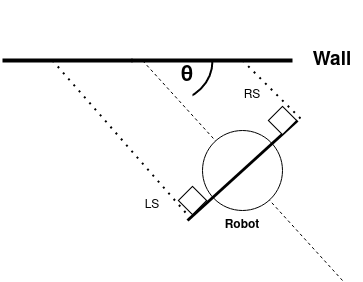
\includegraphics[width=0.6\textwidth]{figures/robotAproachAngle.png}
\caption{\label{figDefAproachAngle}Diagram of the robot approaching an obstacle, defining approach angle.}
\end{figure}

\begin{table}[H]
\caption{\label{tabAproachAngleSensorOut}The Expected Sensor output for various approach angles towards an obstacle, Approach angle \(\theta\) is defined in Figure \ref{figDefAproachAngle}.}
\centering
\begin{tabular}{ll}
\toprule
Approach Angle \(\theta\) & expected Sensor Report\\
\midrule
\(\theta\)<\(\pi\)/2 & LS<RS\\
\(\theta\)>\(\pi\)/2 & LS>RS\\
\(\theta\)=\(\pi\)/2 & LS=RS\\
\bottomrule
\end{tabular}
\end{table}

\subsubsection{Desired behaviour \label{secColisDesiderdBehaviour}}
\label{sec:orgeea829c}
It is obvious that the desired behaviour when approaching an obstacle at an angle is to turn in such a way that the obstacle is no-longer directly in front. It is intuitive to see that the optimal way to turn is always in such a way as to minimise the required angle change. For example the approach angle shown in Figure \ref{figDefAproachAngle} would elicit an intuitive response to turn further left until driving parallel along the wall. The approach angles, their respective sensor readouts and the desired turn can be formulated in Table \ref{tabApproachAngleDesiredBehaviour}.

\begin{table}[H]
\caption{\label{tabApproachAngleDesiredBehaviour}Desired Behaviour For a given approach angle}
\centering
\begin{tabular}{lll}
\toprule
Approach Angle \(\theta\) & expected Sensor Report & Desired Turn Direction\\
\midrule
\(\theta\)<\(\pi\)/2 & LS<RS & Left\\
\(\theta\)>\(\pi\)/2 & LS>RS & Right\\
\(\theta\)=\(\pi\)/2 & LS=RS & Left\\
\bottomrule
\end{tabular}
\end{table}

This table highlights one of the key considerations when designing the collision avoidance system, namely that the frontal approach angel must also elicit a turn in some direction. It is thus decided that the control system will have a tendance to turn in the left direction in the case of a frontal approach.

\paragraph{Turn 'aggressiveness'}
\label{sec:org43063c9}
Given the tank staring nature of the robot, the turn rate may be adjusted from turning on the spot (one wheel forward one back) to turning with a large radius (one wheel stationary one wheel forward). For simplicity these turns will be known as ``hard turn'' and ``slow turn'' respectively.

Through experimentation is established that the turning radius for one wheel forward one stationary is roughly \texttt{0.8m}, while of course the turning circle of one wheel forward one back is \(\approx\) \texttt{0}. This means that an ideal turn would begin upon detecting a sensor reading less than \texttt{0.8m}. If the robot is however within this radius of the wall, and pointing directly at it then it is impossible that this larger turning circle won't intersect the wall. It is therefore required that the robot be able to rotate on the spot when very close to the wall. The desired behaviour may be formulated in the Table below:

\begin{center}
\begin{tabular}{ll}
Absolute Distance & Turn aggressiveness\\
\hline
d>0.8 & No turn\\
0.2<d<0.8 & Slow Turn\\
d<0.2 & Hard Turn\\
\end{tabular}
\end{center}

\paragraph{Amplification of Small differences in sensor measurements}
\label{sec:orgbbfb9c2}


\subsubsection{Collision Sensor Membership Functions}
\label{sec:org01d8b2a}

\begin{figure}[H]
\centering
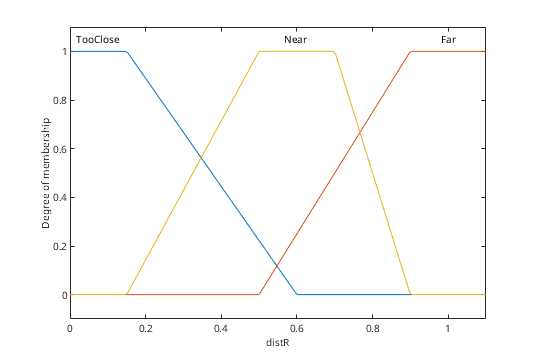
\includegraphics[width=0.6\textwidth]{Section3/Figures/FinalFigures/MembershipFuntionSensor.png}
\caption{\label{figMembershipFunctionFwdSensor}Membership Function for a single forward facing sensor (Bias term=0)}
\end{figure}

\subsubsection{Bias Term Implementation}
\label{sec:org9dbb5e8}
To gain the desired characteristic discussed in Section \ref{secColisDesiderdBehaviour}, it decided that a 'bias' term would be introduced in order to change the symmetry of the sensor feedback membership functions. Since the avoidance behaviour is tuned to respond to differences in sensor readings, this will have the effect, that a front on approach will appear to the controller like an approach of a slight angle and this will induce a turn. The nature of this asymmetry between membership functions is simply a shift along the x axis of \(\Delta x = bias\).

The bias term is applied to the left sensor membership function only and may be negative or positive, resulting in a tendance to turn right or left depending on the sign.

\begin{table}[H]
\caption{\label{tabBiasTermEffect}Effect of varying the value of the bias term assuming a frontal approach.}
\centering
\begin{tabular}{ll}
\toprule
bias value & Turn Tendency\\
\midrule
bias=0 & No tendance\\
bias>0 & Turn Left\\
bias<0 & Turn Right\\
\bottomrule
\end{tabular}
\end{table}

\subsubsection{Membership Function Definition}
\label{sec:org53b9142}
\begin{minted}[breakautoindent=false,style=manni,breaklines=true,linenos=true]{octave}
% Left sensor membership Function (with Bias term)
colisCont = addMF(colisCont,"distL","trapmf", [-10 -10 0.15 0.6+bias],'Name',"TooClose");
colisCont = addMF(colisCont,"distL","trapmf", [0.5+bias 0.9 1.1 2],'Name',"Far");
colisCont = addMF(colisCont,"distL","trapmf", [0.15+bias 0.5+bias 0.7+bias 0.9],'Name',"Near");
% Right sensor membership Function
colisCont = addMF(colisCont,"distR","trapmf", [-10 -10 0.15 0.6],'Name',"TooClose");
colisCont = addMF(colisCont,"distR","trapmf", [0.5 0.9 1.1 2],'Name',"Far");
colisCont = addMF(colisCont,"distR","trapmf", [0.15 0.5 0.7 0.9],'Name',"Near");
\end{minted}

\subsubsection{Collision Avoidance Rules}
\label{sec:orge90c995}
As will be discussed in Section \ref{sectCollisAvoidance}, the collision avoidance rules will operate in a manner completely oblivious to the target seeking steering, as such none of the rules defined below make reference to the angle to target measurement \(\phi\).

\begin{minted}[breakautoindent=false,style=manni,breaklines=true,linenos=true]{octave}
%Turn Right Slow
colisCont = addRule(colisCont,"distL==Near & distR==Far => powerL=Fwd, powerR=Off (1)");
%Turn Left Slow
colisCont = addRule(colisCont,"distL==Far & distR==Near => powerL=Off, powerR=Fwd (1)");
%Turn Left Hard
colisCont = addRule(colisCont,"distL==Near & distR==TooClose => powerL=Rev, powerR=Fwd (1)");
%Turn Right Hard
colisCont = addRule(colisCont,"distL==TooClose & distR==Near => powerL=Fwd, powerR=Rev (1)");
\end{minted}

\subsubsection{Bias Term Implementation}
\label{sec:org28907dc}

\subsection{Way-point Seeking \label{secWaypointSeeking}}
\label{sec:org6fe2cc1}
The way-point seeking controller is also implemented using fuzzy logic. This

\subsubsection{Input}
\label{sec:org47117be}
The input for the way-point seeking algorithm is a derived metric referred to in this report as 'relative heading angle' and denoted by \(\phi\). This angle refers to the angle between the absolute heading of the robot \(\theta\) and the heading angle from the robot to the target (output by the function \texttt{computeHeadingAngle()}).
\begin{figure}[H]
\centering
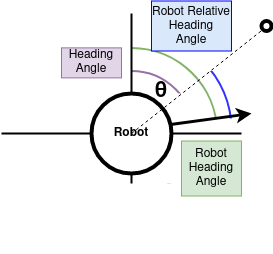
\includegraphics[width=0.6\textwidth]{figures/RobotHeadingAngle.png}
\caption{\label{figDefRelHeadingAngle}Definition of robot relative heading angle \(\phi\)}
\end{figure}

The angle \(\phi\) may be defined according to \ref{eqPhiDef}:

\begin{align}
\label{eqPhiDef}
\phi = RobotHeading -\theta
\end{align}

The code for this is shown below:
\begin{minted}[breakautoindent=false,style=manni,breaklines=true,linenos=true]{octave}
Theta = wrapToPi((newHeadingAngle)-(state(timeStep,stateEnum.angHeading)));
\end{minted}

The \texttt{wrapToPi()} function is used so that the angles returned are always within \textpm{} \(\pi\). This avoids the robot sometimes rotating fully when approaching a target from above.

\subsubsection{Desired behaviour}
\label{sec:org26b31ff}
When \(\phi\) is negative this means the target is to the left of the robot, then when \(\phi\) is positive, this means the target is to the right of the robot. The action in either case is fairly intuitive: when the target is to the right, turn right and when the targe is to the left, turn left. These characteristic rules are shown in

\begin{table}[H]
\caption{\label{tabWaypointSeekingDesiredBehaviour}Desired behaviour for Way-point Seeking algorithm with different values of \(\phi\)}
\centering
\begin{tabular}{ll}
\toprule
\(\phi\) & Turn Direction\\
\midrule
\(\phi\)=0 & No turn (forward motion)\\
\(\phi\)>0 & Turn Right\\
\(\phi\)<0 & Turn Left\\
\bottomrule
\end{tabular}
\end{table}

\paragraph{Dead-zone}
\label{sec:orgf71aee1}
To stop the robot constantly oscillating between turning left and right however, a dead-zone is added in the middle which where acceptably low angles will still elicit forward movement.

\subsubsection{Membership Functions}
\label{sec:org318fe7f}
To get the desired behaviour in Table \ref{tabWaypointSeekingDesiredBehaviour}, three separate membership functions for the input \(\phi\) must exist:
\begin{itemize}
\item \emph{TargetRight}
\item \emph{TargetLeft}
\item \emph{TargetCenter}
\end{itemize}

\begin{figure}[H]
\centering
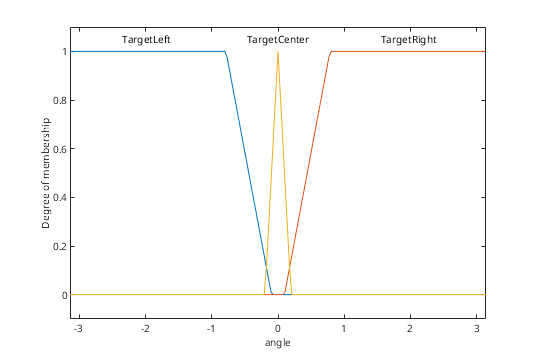
\includegraphics[width=0.6\textwidth]{Section3/Figures/FinalFigures/AngleMembershipFunction.png}
\caption{\label{figMembershipFunctionAngle}Membership Function for relative angle \(\phi\) input, Angle given in Radians.}
\end{figure}

\subsubsection{Collision avoidance prioritisation}
\label{sec:org171ce9a}
The rules to elicit the current turning behaviour by themselves are relatively simple, however it is necessary to consider the condition in which an obstacle is present, which is in-between the robot and the target. In this case the way-point seeking behaviour would be steering the robot towards the wall, while the collision avoidance algorithm would be steering the robot away. The intuitive solution to this problem would be of course to prioritize the collision avoidance steering. To do this the rules defined for the collision avoidance are contingent on both left and right sensor inputs being in the far membership function. Thus when the robot is in open terrain the Waypoint seeking algorithm behaves nominally, however close to an obstacle it will lose it's authority.
\subsubsection{Turn Aggressiveness \label{sectWaypointSeekTurnAgressiveness}}
\label{sec:orgd82fe20}
Since a condition of the robot reaching a way-points is that it get within a tolerance of \texttt{0.05m}, the turning circle guiding the robot must allow for the robot to reach the target to within this tolerance. The robot is not smart enough to first back away from the target and then approach again, rather it will simply, circle the target eternally at the specified turn rate. As such the turn rate must be smaller than the target tolerance meaning that only hard turns are suitible.

\subsubsection{Way-point seeking rules}
\label{sec:org3cb8083}
The following Source code is used to define the way-point seeking rules:

\begin{minted}[breakautoindent=false,style=manni,breaklines=true,linenos=true]{octave}
% Turning (Contingent on Sensor distances being "far")
colisCont = addRule(colisCont,"distL==Far & distR==Far & angle==TargetRight => powerL=Fwd, powerR=Rev (1)");
colisCont = addRule(colisCont,"distL==Far & distR==Far & angle==TargetLeft => powerL=Rev, powerR=Fwd (1)");

% Forward motion in "deadzone" (Contingent on Sensor distances being "far")
colisCont = addRule(colisCont,"distL==Far & distR==Far & angle==TargetCenter=> powerL=Fwd, powerR=Fwd (1)");
\end{minted}

\section{Test Plan}
\label{sec:org54d9795}
\subsection{Collision avoidance tests}
\label{sec:org137e7a9}
Based on the considerations of Sections \ref{sectCollisionAvoidance} and \ref{secWaypointSeeking}, the controller collision avoidance behaviour will be tested. The values for LS and RS corresponding to these conditions are defined and will then be passed into the controller. The resulting output power for each wheel is then tabulated in Table \ref{tabColisAvoidanceTests}.

\begin{table}[H]
\caption{\label{tabColisAvoidanceTests}Tabulated test conditions and resulting output for collision avoidance behaviour}
\centering
\tiny
\begin{tabular}{lrrrrll}
\toprule
Comment \footnotemark & LS & RS & P\_LW & P\_RW & Expected Output & Actual Output\\
\midrule
Preferentially turn left during frontal approach & 0.7 & 0.7 & -0.77 & 3.08 & turn left & turn left\\
Turn Hard Left When \(\theta\)<pi/2 and total distance is small & 0.2 & 0.3 & -4.27 & 3.69 & turn hard left & turn hard left\\
Turn Slow Left When \(\theta\)<pi/2 and total distance is medium & 0.6 & 0.8 & 1.13 & 2.01 & turn slow left & turn slow left\\
Turn Hard Right When \(\theta\)>pi/2 and total distance is small & 0.3 & 0.2 & 1.72 & -3.30 & turn hard right & turn hard right\\
Turn Slow Right When \(\theta\)>pi/2 and total distance is medium & 0.8 & 0.6 & 4.79 & -0.37 & turn slow right & turn slow right\\
\bottomrule
\end{tabular}
\end{table}\footnotetext[1]{\label{org38de3e4}\(\theta\) is defined as the approach angle to a wall}

\subsection{Way-point Steering Test}
\label{sec:orgad1bab9}
\begin{table}[H]
\caption{\label{tabWPAvoidanceTests}Tabulated test conditions and resulting output for Waypoint steering behaviour}
\centering
\tiny
\begin{tabular}{lrrlrrll}
\toprule
Comment & LS & RS & \(\phi\) & P\_RW & P\_LW & Expected Output & Actual Output\\
\midrule
Turn Right when \(\phi\) is positive + no Obstacle & 1 & 1 & \(\pi\)/8 & 8.0391 & -5.5654 & turn hard right & turn hard right\\
Turn Left when \(\phi\) is negative + no Obstacle & 1 & 1 & -\(\pi\)/8 & -5.5654 & 8.0391 & turn hard left & turn hard left\\
\bottomrule
\end{tabular}
\end{table}

\section{Results}
\label{sec:org5ce204a}
\subsection{Final Path No Walls}
\label{sec:org88d3e44}
Figure \ref{figWaypointFollowingRobotNoObstacles} shows the path of the robot when seeking the way-points shown in Table \ref{tabWaypointsFollowed}.

\begin{table}[H]
\caption{\label{tabWaypointsFollowed}Waypoints followed by robot}
\centering
\begin{tabular}{rrr}
\toprule
Point & X & Y\\
\midrule
1 & 1 & 2\\
2 & 1.5 & 1\\
3 & 3 & -2\\
4 & -1 & -2\\
5 & -0.7 & -0/7\\
\bottomrule
\end{tabular}
\end{table}

\begin{center}
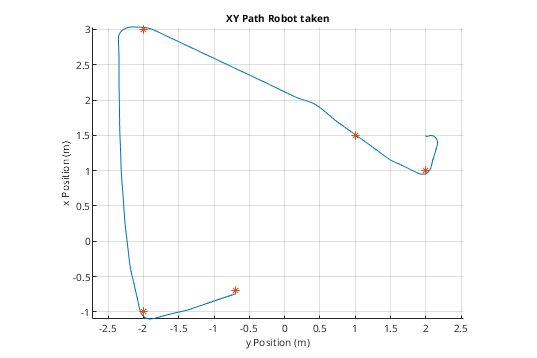
\includegraphics[width=0.6\textwidth]{Section3/Figures/FinalFigures/xVyCustom_HomingWP_Task1nowalls.png}
\end{center}

\subsection{Final Path With Walls}
\label{sec:org48932fc}
Figure \ref{figWaypointsFollowingWithObstacles} shows the path of the robot with obstacles present following the way-points shown in Table \ref{tabWaypointsFollowedWithObstacles}.

\begin{table}[H]
\caption{\label{tabWaypointsFollowedWithObstacles}Waypoints followed by robot in test with obstacles.}
\centering
\begin{tabular}{rrr}
\toprule
Point & X & Y\\
\midrule
Start & -1 & 0\\
123 & 2 & 3\\
214 & 1 & 4\\
3 & 3 & -4\\
4 & -1 & -2\\
5 & 3 & 0\\
End & 1.5 & 2\\
\bottomrule
\end{tabular}
\end{table}

\begin{figure}[H]
\centering
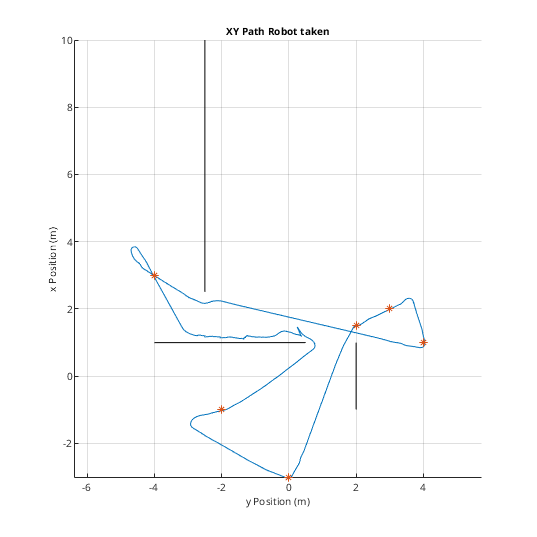
\includegraphics[width=0.6\textwidth]{Section3/Figures/FinalFigures/xVyCustom_HomingWP_Task2task2Walls.png}
\caption{\label{figWaypointsFollowingWithObstacles}XY Path of Waypoint Seeking robot with obstacles present}
\end{figure}

\section{Discussion}
\label{sec:org0c4017b}
\subsection{'Wall Scrape' With obstacles \label{wallScrape}}
\label{sec:org5693532}
One particularly difficult scenario for the robot to deal with is when there is a wall in-between itself and the target, at this point the way-point steering starts to fight with the collision avoidance steering since the former wishes to steer through the wall, while the latter wishes to push away from the wall. Since, by design, the way-point guidance loses it's authority when close to the wall, this results in an angular 'wobbling' as the obstacle avoidance algorithm turns away from the wall and target until the sensor readings are suitable low for the way-point guidance to kick in again and steer back towards the wall. Since the Way-point steering turns with one wheel forward and one wheel back, this means that as soon as it kicks in the entire forward motion of the Robot is arrested, meaning that motion along such a wall results not only the angular oscillation, but also on a jerky forward motion.

The angular oscillation can be seen in Figure \ref{figAngluarOscilationWallScrape} between t=25-45s \footnote{Note that discontinuities in this plot are due to the angle wrapping from \textpm{} \(\pi\)}.

\begin{figure}[H]
\centering
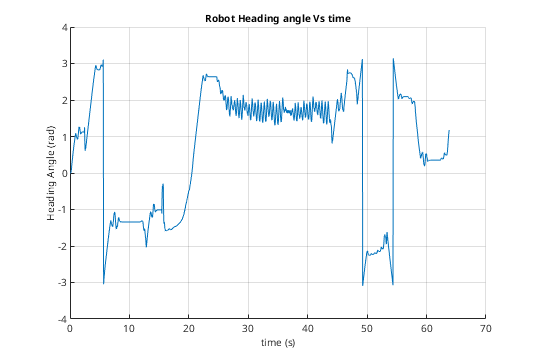
\includegraphics[width=0.6\textwidth]{Section3/Figures/FinalFigures/psiVtCustom_HomingWP_Task2task2Walls.png}
\caption{\label{figAngluarOscilationWallScrape}The angular oscillating Resulting from Wall Scrape}
\end{figure}

\section{Improvements}
\label{sec:orgcc22daa}
\subsection{Acting on \(\Delta\) Distance}
\label{sec:orga60a253}
The desired behaviour of the collision avoidance algorithm is effectively to maximise the difference between the two sensors, since this is the effect that turning has. Perhaps a better suited input for the controller is the difference between the right and left sensor rather than the absolute value of both. This might allow for a more consice set of rules, since it boils down two separate inputs with their own rule sets into just one.

\subsection{Acting on absolute distance to target}
\label{sec:orgf1f774b}
One mitigation for the 'wall scrape' described in Section \ref{wallScrape} might be to have different turn aggressiveness depending on the relative distance to the target. As discussed in Section \ref{sectWaypointSeekTurnAgressiveness}, the tank steering is required to avoid the case in which the robot is close enough to the target that it's turning doing a slow turn would not allow it to intersect the target. This condition only exists however if the target is within the robot's turning circle, so if the distance to the targe could also be used as an input, this could be used as a switch between hard turning and slow turning. Since slow turning just involves stopping/Slowing one wheel relative to the other rather than driving it backwards, this might act to reduce the 'jerkiness' of the motion along a wall.

\section{Appendices}
\label{sec:org36f3313}
\end{document}
